Subimos un objeto de 12 kg por una rampa inclinada 30$^\circ$ hasta una altura de 14 m. ¿Qué energía potencial tendrá al llegar arriba?


\begin{minipage}{0.3\textwidth}
    \begin{figure}[H]
        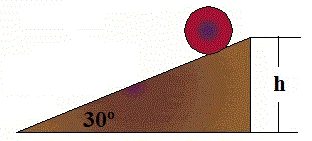
\includegraphics[width=\linewidth]{../images/ejercicio-energia-potencial-rampa}
    \end{figure}
\end{minipage}\hfill
\begin{minipage}{0.65\textwidth}
    \begin{solutionbox}{5.3cm}
        \begin{multicols}{2}
            Datos:

            E$_p$ = ?

            h = 14 m

            g= 9.8 m/s$^2$

            m = 12 kg

            La energía potencial es:
            \[E_p=mgh\]

            \vspace{2cm}

            Sustituyendo nuestros datos en la fórmula:
            \[
                \begin{array}{rl}
                    E_p & = (12 \text{ kg})(9.8 \text{ m/s$^2$})(14 \text{ m}) \\[1em]
                        & =1646.4 \text{ J }
                \end{array}
            \]

        \end{multicols}
        \begin{center}La energía potencial del objeto es de 1646.4 Joules.\end{center}
    \end{solutionbox}
\end{minipage}